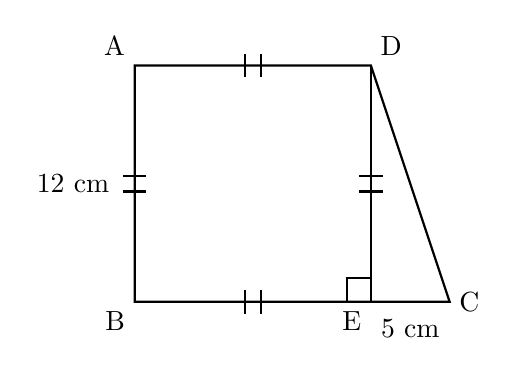
\begin{tikzpicture}[scale=1]

    % Define the coordinates of the vertices
    \coordinate (A) at (0,3);
    \coordinate (B) at (0,0);
    \coordinate (E) at (3,0);
    \coordinate (C) at (4,0);
    \coordinate (D) at (3,3);

    % Draw the main polygon (Trapezoid ABCD)
    \draw[thick] (A) -- (B) -- (C) -- (D) -- cycle;

    % Draw the altitude DE
    \draw[thick] (D) -- (E);

    % Add right angle symbol at E
    \draw[thick] (2.7,0) -- (2.7,0.3) -- (3,0.3);

    % Add equality tick marks on the sides of the square ABED
    % Tick marks on AB
    \draw[thick] (-0.15,1.4) -- (0.15,1.4);
    \draw[thick] (-0.15,1.6) -- (0.15,1.6);
    
    % Tick marks on AD
    \draw[thick] (1.4,2.85) -- (1.4,3.15);
    \draw[thick] (1.6,2.85) -- (1.6,3.15);

    % Tick marks on DE
    \draw[thick] (2.85,1.4) -- (3.15,1.4);
    \draw[thick] (2.85,1.6) -- (3.15,1.6);
    
    % Tick marks on BE
    \draw[thick] (1.4,-0.15) -- (1.4,0.15);
    \draw[thick] (1.6,-0.15) -- (1.6,0.15);

    % Label the vertices
    \node[above left] at (A) {A};
    \node[below left] at (B) {B};
    \node[right] at (C) {C};
    \node[above right] at (D) {D};
    \node[below left] at (E) {E};

    % Add measurements
    \node[left] at (-0.2,1.5) {$12$ cm};
    \node[below] at (3.5,-0.1) {$5$ cm};

\end{tikzpicture}